% \documentclass[oneside,11pt]{book}

% \ifdefined\correction
  % \usepackage[noenonce, correction, source, ds]{style}
% \else
  % \usepackage[enonce, nocorrection, ds]{style}
% \fi

% \usepackage{alphabet}

% \DeclareMathOperator{\lcoef}{cd}

% \begin{document}
% %%%%%%%%%%%%%%%%%%%%%%%%%%%%%%%%%%%%%%%%%%%%%%%%%%%%
% \etablissement{Stanislas}
% \date{09 novembre 2019}
% \niveau{PSI}
% \module{DS~n°03}
% \titre{Devoir Surveillé}
% \soustitre{4h}
% \author{A. Camanes}
% % \deadline{}
% \entete
% \renewcommand{\labelitemi}{$\bullet$}
% \renewcommand{\labelitemii}{$\ast$}
% %%%%%%%%%%%%%%%%%%%%%%%%%%%%%%%%%%%%%%%%%%%%%%%%%%%%

{\ifenonce
\begin{center}
Ce sujet est composé de \gras{deux} problèmes \gras{indépendants}.
\end{center}
\fi}


%=============

\begin{probleme}[Une famille d'intégrales généralisées]
Pour $\ag$ réel et $n$ entier strictement positif, on considère les intégrales généralisées :
\[
I_{n,\ag} = \dint_0^{+\infty} \frac{(\sin t)^n}{t^\ag} \dt
\]
Une intégrale généralisée est semi-convergente si elle est convergente mais non absolument convergente.

%=======
\partie{Le cas $n = 1$}
\qu Étude de la convergence de $I_{1,\ag} = \dint_0^{+\infty} \frac{\sin t}{t^\ag} \dt$.
\squ On suppose $\ag > 1$. Étudier la convergence absolue de l'intégrale.

\squ On suppose $0 < \ag \leq 1$.
\ssqu Montrer que l'intégrale $I_{1,\ag}$ converge.
\indic{On pourra utiliser une intégration par parties pour l'étude au voisinage de l'infini.}

\ssqu On considère la série de terme général $u_n = \dint_{n\pi}^{(n+1)\pi} \frac{\sin t}{t^\ag} \dt$. Montrer que
\[
\frac{2}{(n+1)^\ag \pi^\ag} \leq \abs{u_n} \leq \frac{2}{n^\ag \pi^\ag}.
\]

\ssqu Que peut-on en déduire sur la convergence de $\dint_0^{+\infty} \abs{\frac{\sin t}{t^\ag}} \dt$ et de $I_{1,\ag}$ ?

\squ On suppose $\ag \leq 0$. On considère la suite $v_n = \dint_\pi^{n \pi} \frac{\sin t}{t^\ag} \dt$. Étudier la limite de $(\abs{v_{n+1} - v_n})$ et en déduire la nature de l'intégrale $I_{1,\ag}$.

\qu Pour tout $(a, b) \in \R^2$, on considère l'intégrale
\[
J_{a,b} = \dint_0^{+\infty} t^b \sin(t^a) \dt
\]
et on note
\begin{itemize}
\item $D_1$ l'ensemble des couples $(a, b)$ tels que $J_{a,b}$ soit absolument convergente,
\item $D_2$ l'ensemble des couples $(a, b)$ tels que $J_{a,b}$ soit semi-convergente,
\item $D_3$ l'ensemble des couples $(a, b)$ tels que $J_{a,b}$ soit divergente.
\end{itemize}
À tout couple $(a, b)$ on associe dans le plan un point $M$ de coordonnées $(a, b)$. Représenter graphiquement les domaines $D_1$, $D_2$ et $D_3$ dans un même système d'axes.

%=======
\partie{Le cas $n = 3$, $\ag = 2$}
\qu Étudier la convergence de $I_{3,2}$.

\Qu Soit $f : ]0,\pi/2] \to \R,\, t \mapsto \frac{\sin t}{t}$. Étudier le sens de variation de $f$.

\squ Soit $F_{a,b}(x) = \dint_{a x}^{b x} \frac{\sin t}{t^2} \dt$. Montrer que la limite de $F_{a,b}(x)$ lorsque $x$ tend vers $0$ vaut $\ln \frac{b}{a}$.

\qu Soit $I(\eg) = \dint_\eg^{+\infty} \frac{\sin^3 t}{t^2} \dt$.
\squ Montrer que $I(\eg) = k F_{1,3}(\eg)$ où $k$ est une constante que l'on déterminera.

\squ En déduire la valeur de $I_{3,2}$.

%=======
\partie{Le cas $\ag = n$}
On pose $A_n = I_{n,n} = \dint_0^{+\infty} \left(\frac{\sin t}{t}\right)^n \dt$. On admet que $A_1 = \frac{\pi}{2}$.
\qu Pour tout réel $x$ strictement positif, calculer $G(x) = \dint_0^{+\infty} \frac{\sin(x t)}{t} \dt$.

\qu Étudier la convergence de l'intégrale $A_n$ pour tout $n$ supérieur ou égal à $2$.

\qu Calculer $A_2$.

\qu Exprimer $A_4$ en fonction de $A_2$ et en déduire la valeur de $A_4$.
\end{probleme}

\begin{solution}[Solution du Problème]
\concours{ENSAIT - MP - 1996 (épreuve de $2$h)}

%=============
\partiesimple{Remarques}
% \qu Trop de copies manquent de liant : les phrases doivent être complètes (sujet + verbe + complément).

\qu La manipulation des inégalités, des valeurs absolues et des signes est souvent mal maîtrisée. La valeur absolue est décroissante sur $\R_-$ et croissante sur $\R_+$. Il convient d'expliquer, sans ambiguïté, comment le calcul est mené de manière à convaincre le correcteur que cette notion est acquise.

\qu La relation d'équivalence doit être utilisée avec rigueur, mais sans craintes.

\qu Bien souvent, une inégalité était tout aussi efficace qu'un calcul de $o$.

\qu Il est important de prouver la convergence d'une intégrale, l'existence d'une limite,\ldots\, avant de commencer à calculer avec.

\qu L'étude de l'intégrale $J_{a,b}$ doit être ramenée à celle de $I_{1,\ag}$ pour pouvoir mener la disjonction de cas. Peu de copies ont abordé cette question.

\qu L'étude de fonction de la question \gras{4.a)} doit être menée avec soin.

\setcounter{cqu}{0}

%=======
\partie{$n = 1$}
\Qu La fonction $f : t \mapsto \frac{\sin t}{t^\ag}$ est continue sur $]0, +\infty[$.

\gras{Étude en $0$.} D'après les équivalents classiques,
\[
\frac{\sin t}{t^\ag} \sim_0 \frac{t}{t^\ag} \sim_0 \frac{1}{t^{\ag-1}}
\]
Ainsi, en utilisant le théorème de comparaison des fonctions à valeurs positives, $\dint_0^1 \abs{f(t)} \dt$ converge si et seulement si $\ag - 1 < 1$, i.e. $\ag < 2$. De plus, comme $t \mapsto \frac{\sin t}{t^\ag}$ est positive sur un voisinage de $0$, alors il s'agit d'une condition nécessaire et suffisante de convergence sur un voisinage de $0$.

\gras{Étude en $+\infty$.} D'après les propriétés de la fonciton sinus,
\[
\pourtout t \in [1,+\infty[,\, \abs{f(t)} \leq \frac{1}{t^\ag}
\]
Comme $\ag > 1$, d'après les intégrales de Riemann, $\dint_1^{+\infty} \frac{1}{t^\ag} \dt$ converge. Ainsi, $f$ est intégrable sur $[1,+\infty[$.

Finalement, lorsque $\ag > 1$, l'intégrale $\dint_0^{+\infty} f(t) \dt$ converge absolument si et seulement si $\ag \in ]1, 2[$.

\squ
\ssqu La fonction $f : t \mapsto \frac{\sin t}{t^\ag}$ est continue sur $]0, +\infty[$.

\gras{Étude en $0$.} D'après les équivalents classiques,
\[
\frac{\sin t}{t^\ag} \sim_0 \frac{t}{t^\ag} \sim_0 \frac{1}{t^{\ag-1}}
\]
Comme $\ag < 1$, alors $\dlim_{t\to0} f(t) = 0$. Ainsi, $f$ est prolongeable par continuité en $0$ et $\dint_0^1 f(t) \dt$ converge.

\gras{Étude en $+\infty$.} Les fonctions $t \mapsto -\cos(t)$ et $t \mapsto \frac{1}{t^\ag}$ sont de classe $\CC^1$ sur $[1,+\infty[$. De plus, $\dlim_{t\to+\infty} \frac{\cos(t)}{t^\ag} = 0$. Ainsi, d'après la formule d'intégration par parties généralisée, $\dint_1^{+\infty} \frac{\sin t}{t^\ag} \dt$ est de même nature que $\dint_1^{+\infty} \frac{\cos(t)}{t^{\ag+1}} \dt$. Or, $\abs{\frac{\cos(t)}{t^{\ag+1}}} \leq \frac{1}{t^{\ag+1}}$ et, d'après les intégrales de Riemann, $\dint_1^{+\infty} \frac{1}{t^{\ag+1}} \dt$ converge. Ainsi, $\dint_1^{+\infty} \frac{\sin t}{t^{\ag}} \dt$ est convergente.

Finalement, $I_{1,\ag}$ est convergente.

\ssqu En utilisant le changement de variable affine $\phi : u \mapsto u + n \pi$,
\begin{align*}
u_n &= \dint_0^\pi \frac{\sin(n \pi + u)}{(n \pi + u)^\ag} \du\\
&= (-1)^n \dint_0^\pi \frac{\sin(u)}{(n \pi + u)^\ag} \du
\end{align*}
De plus, la fonction sinus est positive sur $[0,\pi]$ et $\dint_0^\pi \sin(t) \dt = 2$. Ainsi, en utilisant la décroissance de $u \mapsto \frac{1}{(n \pi + u)^\ag}$ et la croissance de l'intégrale,
\[
\frac{2}{(n+1)^\ag \pi^\ag} \leq \abs{u_n} \leq \frac{2}{n^\ag \pi^\ag}
\]

\ssqu Lorsque $\ag \leq 1$, le théorème sur les séries de Riemann assure que $\dsum \frac{1}{(n+1)^\ag}$ diverge. Ainsi, $\dsum \abs{u_n}$ diverge.

Ainsi, en utilisant la relation de Chasles et le signe de la fonction sinus sur les intervalles de la forme $[n\pi, (n+1)\pi]$,
\begin{align*}
\dint_0^{(n+1)\pi} \abs{\frac{\sin t}{t^\ag}} \dt &= \dsum_{k=0}^n \dint_{k\pi}^{(k+1)\pi} \abs{\frac{\sin t}{t^\ag}} \dt \\
&= \dsum_{k=0}^n \abs{u_k}
\end{align*}
Comme $\dsum \abs{u_k}$ diverge, alors $\dint_0^{+\infty} \abs{\frac{\sin t}{t^\ag}} \dt$ diverge.

Finalement, d'après \gras{i.}, $I_{1,\ag}$ est convergente et, d'après \gras{iii} elle n'est pas absolument convergente. Ainsi, lorsque $\ag \in ]0,1]$, $I_{1,\ag}$ est semi-convergente.

\squ D'une part, $t \mapsto \frac{\sin t}{t^\ag}$ est continue sur $]0,\infty[$ et prolongeable par $0$ en $0$. On étudie donc la nature de l'intégrale sur $[\pi, +\infty[$.

Soit $n \in \N^*$. D'après le calcul de la question précédente,
\begin{align*}
\abs{v_{n+1} - v_n} &= \dint_0^\pi \frac{\sin u}{(n\pi+u)^\ag} \du \\
&\geq \frac{2}{((n+1) \pi)^\ag}
\end{align*}
Ainsi, si $\ag < 0$, alors $\dlim_{n\to+\infty} \abs{v_{n+1} - v_n} = +\infty$ et $(v_n)$ diverge. Lorsque $\ag = 0$, la suite est constante égale à $2$.

Si $I_{1,\ag}$ convergeait, alors $(v_n)$ admettrait une limite en $+\infty$ et $(v_{n+1} - v_n)$ tendrait vers $0$. Ainsi, $I_{1,\ag}$ diverge.

\qu Commençons par résumer les calculs précédents.
\begin{itemize}
\item Si $1 < \ag < 2$, alors $I_{1,\ag}$ est absolument convergente.
\item Si $0 < \ag \leq 1$, alors $I_{1,\ag}$ est semi-convergente.
\item Si $\ag \leq 0$ ou $\ag \geq 2$, alors $I_{1,\ag}$ est divergente.
\end{itemize}

\medskip

Si $a = 0$, alors $J_{0,b} = \dint_0^{+\infty} t^b \sin(1) \dt$ est une intégrale de Riemann divergente.

La fonction $u \mapsto u^{1/a}$ est $\CC^1$ et bijective sur $\R_+^*$. Ainsi, d'après le théorème de changement de variables, $J_{a,b}$ est de même nature que
\[
I_{1,\frac{a-b-1}{a}} = \dint_0^{+\infty} u^{b/a} \sin(u) \frac{u^{1/a-1}}{a} \du
\]
Si $a > 0$, on obtient ainsi les cas suivants :
\begin{itemize}
\item Si $-1-a<b<-1$, alors $J_{a,b}$ est absolument convergente.
\item Si $-1<b<a-1$, alors $J_{a,b}$ est semi-convergente.
\item Si $b \leq -a-1$ ou $b \geq a - 1$, alors $J_{a,b}$ est divergente.
\end{itemize}

Si $a \leq 0$, on obtient les cas suivant:
\begin{itemize}
\item Si $-1 < b < -1-a$, alors $J_{a,b}$ est absolument convergente.
\item Si $a-1 < b < -1$, alors $J_{a,b}$ est semi-convergente.
\item Si $b \geq -a-1$ ou $b \leq a - 1$, alors $J_{a,b}$ est divergente.
\end{itemize}

Ces résultats peuvent être résumés dans le graphe suivant.
\begin{center}
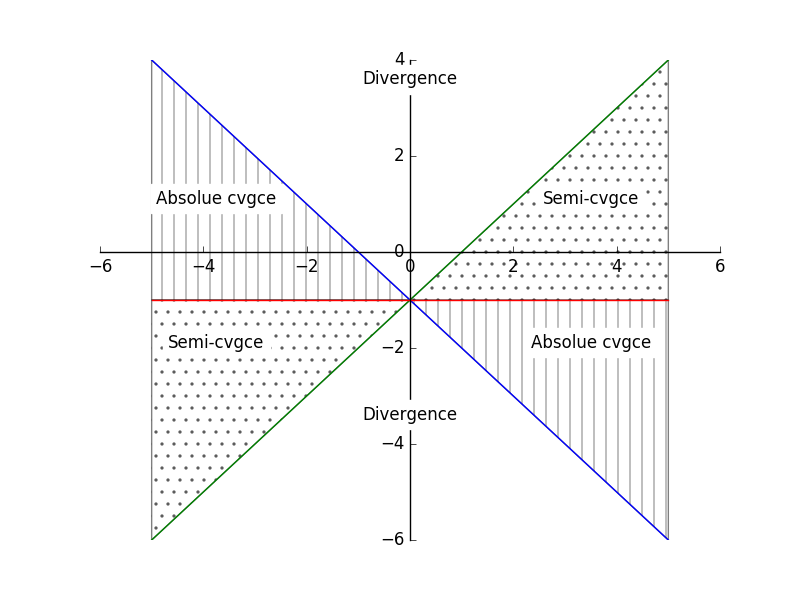
\includegraphics[width=0.45\textwidth]{ensait-1996-domaines.png}
\end{center}

%=======
\partie{$n = 3$, $\ag = 2$}
\qu La fonction $f : t \mapsto \frac{\sin^3(t)}{t^2}$ est continue sur $\R_+^*$.

\gras{Étude en $0$.} Comme $f(t) \sim_0 t$, la fonction $f$ est prolongeable par continuité en $0$. Ainsi, $\dint_0^1 f(t) \dt$ converge.

\gras{Étude en $+\infty$.} D'après les propriétés du sinus, $\abs{f(t)} \leq 1/t^2$. Ainsi, par comparaison à une intégrale de Riemann, $\dint_1^{+\infty} f(t) \dt$ converge.

Finalement, $I_{3,2}$ converge.

\Qu La fonction $f$ est dérivable sur $]0,\pi/2]$ et pour tout $t \in ]0,\pi/2[$,
\[
f'(t) = \frac{t \cos(t) - \sin(t)}{t^2} = \cos(t) \frac{t - \tan(t)}{t^2}
\]
Posons $\phi : t \mapsto t - \tan(t)$. Alors, $\phi' : t \mapsto -\tan^2(t)$ est négative donc $\phi$ est décroissante. Comme $\phi(0) = 0$, alors $f'$ est négative donc $f$ est décroissante.

\squ Pour $x$ assez petit, $[a x, b x] \subset [0,\pi/2]$. Ainsi, en utilisant les variations de la fonction $f$,
\[
\frac{f(a x)}{t} \leq \frac{\sin t}{t^3} \leq \frac{f(b x)}{t}
\]
D'après la croissance de l'intégrale,
\[
f(a x) \ln \frac{b}{a} \leq F_{a,b}(x) \leq f(b x) \ln \frac{b}{a}
\]
Comme $\dlim_{u\to 0} f(u) = 1$, d'après le théorème d'encadrement, $\dlim_{x\to 0} F_{a,b}(x) = \ln \frac{b}{a}$.

\gras{$2$ème méthode.} En effectuant des études de fonctions, on montre que pour tout $t$ réel,
\[
t - \frac{t^3}{6} \leq \sin(t) \leq t
\]
Ainsi,
\[
\frac{1}{t} - \frac{t^2}{6} \leq \frac{\sin(t)}{t^2} \leq \frac{1}{t}
\]
et
\[
\ln\frac{b}{a} - \frac{(b^3 - a^3) x^3}{18} \leq F_{a,b}(x) \leq \ln\frac{b}{a}
\]

\Qu En utilisant les formules de linéarisation,
\[
\sin^3(t) = \frac{3}{4} \sin(t) - \frac{1}{4} \sin(3 t)
\]
Or, en reprenant une comparaison à une intégrale de Riemann, les fonctions $t \mapsto \frac{\sin(t)}{t^2}$ et $t \mapsto \frac{\sin(3 t)}{t^2}$ sont intégrables sur $[\eg, +\infty[$. Ainsi, d'après la linéarité des intégrales convergentes puis un changement de variable affine,
\begin{align*}
I(\eg) &= \frac{3}{4} \dint_\eg^{+\infty} \frac{\sin(t)}{t^2} \dt - \frac{1}{4} \dint_\eg^{+\infty} \frac{\sin(3 t)}{t^2} \dt \\
&= \frac{3}{4} \dint_\eg^{+\infty} \frac{\sin(t)}{t^2} \dt - \frac{3}{4} \dint_{3 \eg}^{+\infty} \frac{\sin(u)}{u^2} \dt \\
&= \frac{3}{4} F_{1,3}(\eg)
\end{align*}

\squ D'après la question précédente, comme $I_{3,2}$ est convergente, $I_{3,2} = \dlim_{\eg\to 0} I(\eg)$ et
\[
I_{3,2} = \frac{3}{4} \ln(3)
\]

%=======
\partie{$\ag = n$}
\qu En effectuant le changement de variable affine $\phi : u \mapsto \frac{u}{x}$,
\[
G(x) = \dint_0^{+\infty} \frac{\sin(x t)}{t} \dt = \dint_0^{+\infty} \frac{\sin(u)}{u} \du = \frac{\pi}{2}
\]

\qu La fonction $f : t \mapsto \left(\frac{\sin t}{t}\right)^n$ est continue sur $\R_+^*$.

\gras{Étude en $0$.} Comme $f(t) \sim 1$, la fonction $f$ est prolongeable par continuité en $0$ et $\dint_0^1 f(t) \dt$ converge.

\gras{Étude en $+\infty$.} Soit $n \geq 2$. Alors, $\abs{f(t)} \leq 1/t^2$ et $\dint_1^{+\infty} f(t) \dt$ converge.

Finalement, $A_n$ est bien définie.

\qu Les fonctions $t \mapsto \sin^2(t)$ et $t \mapsto -1/t$ sont de classe $\CC^1$ sur $]0, +\infty[$. De plus, $\dlim_{t\to0} \frac{\sin^2(t)}{t} = \dlim_{t\to+\infty} \frac{\sin^2(t)}{t} = 0$. Ainsi, d'après la formule d'intégration par parties,
\[
A_2 = \dint_0^{+\infty} \frac{2 \sin(t) \cos(t)}{t} \dt = G(2) = \frac{\pi}{2}
\]

\qu Les fonctions $t \mapsto \sin^4(t)$ et $t \mapsto -\frac{1}{3t^3}$ sont de classe $\CC^1$ sur $]0, +\infty[$ et leur crochet tend vers $0$. D'après la formule d'intégration par parties,
\[
A_4 = \frac{4}{3} \dint_0^{+\infty} \frac{\cos(t) \sin^3(t)}{t^3} \dt
\]

De même, les fonctions $t \mapsto \cos(t) \sin^3(t)$ et $t \mapsto -\frac{1}{2 t^2}$ sont de classe $\CC^1$ sur $]0, +\infty[$ et leur crochet tend vers $0$. Ainsi, d'après la formule d'intégration par parties,
\begin{align*}
A_4 &= \frac{2}{3} \dint_0^{+\infty} \frac{-\sin^4(t) + 3 \cos^2(t) \sin^2(t)}{t^2} \dt \\
&= \frac{2}{3} \dint_0^{+\infty} \frac{3 \cos^2(t) \sin^2(t) - (1 - \cos^2(t)) \sin^2(t)}{t^2} \dt \\
&= \frac{8}{3} \dint_0^{+\infty} \frac{\cos^2(t) \sin^2(t)}{t^2} \dt - \frac{2}{3} A_2 \\
&= \frac{2}{3} \dint_0^{+\infty} \frac{\sin^2(2t)}{t^2} \dt - \frac{2}{3} A_2 \\
&= \frac{4}{3} \dint_0^{+\infty} \frac{\sin^2(u)}{u^2} \du - \frac{2}{3} A_2 \\
&= \frac{2}{3} A_2 \\
&= \frac{\pi}{3}
\end{align*}
\end{solution}
% \end{document}
